% Metoddelen redogör för vad du gjort och hur du gått tillväga; det är
% en beskrivning av den metod som ligger till grund för det du kommit
% fram till och hävdar i din rapport.

% Beskrivningen i metoddelen ska vara koncis snarare än helt
% uttömmande men ska samtidigt göra det möjligt att upprepa studien

% Metoddelen ska inte vara en omgjord labbinstruktion och den ska inte
% heller innehålla teori med mindre än att teoretiska hänsyn har haft
% en direkt inverkan på metoden.

% Metoddelen skrivs nästan alltid i dåtid (imperfekt) och ofta används
% passiv form för att beskriva forskningsaktiviteter.

\chapter{Genomförande}

Projektets genomförande bestod av fyra delar. Den största delen var
konstruktionen av själva läromaterialet i vilken det ingick sökande efter lämpliga
områden, implementation av domänspecifika språk och skrivande av lärotext. De
tre andra delarna var publicering av läromaterialet på en hemsida, återkoppling på
läromaterialet med en testgrupp samt möten med Åke Fäldt, examinator och
föreläsare för Fysik för ingenjörer. Mötena med Fäldt hade två syften: att hitta
problemområden i fysikkursen och att få återkoppling på läromaterialet. Alla de
olika delar i projektet genomfördes samtidigt men de finns här beskrivna
separat.

\section{Konstruktion av läromaterialet}\label{sec:konstruktion}

Läromaterialet består av fem kapitel som vardera behandlar separata områden.
Skapandet av dem skedde fristående men de innehöll alla de tre faserna sökande,
implementation och skrivande, som såg likartade ut för dem alla. Det fanns dock
visst överlapp mellan de fristående processerna. Sökandet gav ofta flera områden
samtidigt och implementation och skrivande genomfördes ofta parallellt. För att
tydliggöra processerna är de dock beskrivna separat.

\subsection{Sökande efter områden att behandla}\label{sec:valet}

Ett domänspecifikt språk modellerar ett specifikt och avgränsat område. Därför
var det naturligt att söka och tänka i termer av avgränsade områden inom
fysiken.
För att rent praktiskt hitta områden att behandla kontaktades Åke
Fäldt. Dessutom studerades kursens bok (University
Physics~\cite{UP}) och dess övriga material. Av speciellt intresse
var de kapitel som behandlade mekanik (i enlighet med projektets mål att börja
med klassisk mekanik), de områden Fäldt pekat ut som svåra för studenter samt de kapitel som använde sig av en
specifik syntax. Domänspecifik syntax var av intresse att finna
då en betydlig del av domänspecifika språk är modellering av just syntaxen. Denna sökandeprocess innefattade inte bara att \textit{hitta} fysikaliska
områden utan även att \textit{organisera} dem i relation till varandra, för att kunna implementera dem på ett bra sätt och presentera dem i en pedagogisk ordning.

% \subsubsection*{Kontakt med fysikläraren}
% \label{sec:kontakt_faldt}
%
% Fäldt tillfrågades om vilka områden han i allmänhet anser att studenter har
% svårt för. Detta för att i enlighet med projektets mål börja med de, för
% studenterna, problematiska områdena. Enligt Fäldt är ett allmänt problem att
% egna mentala modeller för problem är felaktiga eftersom studenter ofta tar
% genvägar som inte bygger på saker de är säkra stämmer. En annan erfarenhet
% är att så länge den första raden i en uppgiftslösning är rätt, så brukar
% resten också vara rätt. Med andra ord, har studenten väl identifierat vilken typ av
% problem det rör sig om brukar det inte vara några svårigheter att lösa
% uppgiften. Sist men inte minst ansåg Fäldt att det fattades grundläggande
% kunskaper om matematisk analys hos studenterna.
%
% Med hjälp av insikterna från Fäldt drogs två slutsatser. Den första slutsatsen
% var att matematisk analys var ett område värt att behandla i detalj. Den andra
% var att genom att ge struktur till olika typer av problem kan det
% förhoppningsvis underlätta för studenter att lära sig identifiera vilken
% typ av uppgift de handskas med.

% Sökandet i kursboken och kursmaterialet gav viktiga kunskaper om områden att
% behandla. Men minst lika viktiga var de inledande experiment som gjordes på
% varje område för att se huruvida det lämpade sig att göra ett domänspecifikt
% språk av och hur det skulle kunna se ut. Experimenten visade att enbart vissa
% områden, till exempel vektorer, fungerade bra att göra ett domänspecifikt språk
% av. Andra områden, till exempel lutande plan, var mindre lämpliga. Vad som
% skiljer dem åt är att vektorer har tydliga data och operationer (till exempel
% skalärprodukt) medan lutande plan har egenskaper (till exemel
% friktionskoefficienter och vinklar) som är relaterade till varandra med
% ekvationer. Det här diskuteras utförligare i avsnitt~\ref{sec:lampligt}. Det
% framgick också att det blev ett överlapp mellan olika domänspecifika språk trots
% att områdena var fristående.
% Ett exempel var det domänspecifika språk för partikelmekanik som till stor del
% liknade de domänspecifika språken för matematisk analys och vektorer.

% Det blev av dessa skäl nödvändigt att göra en distinktion mellan två typer av
% områden: \textit{grundläggande} och \textit{komposita}. Grundläggande områden är
% helt fristående från andra områden och behandlar grundläggande koncept.
% Komposita områden bygger vidare på andra områden eller tillämpar andra områden
% på konkreta fysikaliska problem.

% \subsubsection*{Områden som valdes ut}
%
% När kunskap inhämtats om olika områden kunde ett urval göras. De områden som
% identifierades som grundläggande och som hade en väl lämpad struktur enligt
% avsnittet innan valdes ut. Med detta som grund blev områdena som valdes ut
% fysikaliska dimensioner, matematisk analys och vektorer. Här följer en
% kortfattad motivering av valet av dem.
%
% \textit{Dimensioner} eftersom det är viktigt för studenter att förstå
% hur dimensioner påverkas av algebraiska operationer. Det kan också vara
% hjälpsamt att utföra automatisk, datorassisterad dimensionsanalys på
% beräkningar. Dimensionsanalys var ett område som Fäldt nämde att studenter
% inte lade tillräckligt mycket vikt vid.
%
% \textit{Matematisk analys} eftersom alla koncept inom klassisk mekanik är
% relaterade genom matematisk analys. Mer specifikt används
% differenser\footnote{Till exempel används $\Delta(x)$ för att beskriva
% förflyttning i $x$-led.} för att beskriva medelrörelse, och infinitesimaler
% för att beskriva momentanrörelser. Vidare var matematisk analys också ett
% område som Fäldt pekade ut som speciellt viktigt och något som studenter har
% svårt för.
%
% \textit{Vektorer} eftersom det är en viktig grundsten inom den klassiska
% mekaniken. Alla krafter, hastigheter och accelerationer betraktas som vektorer i
% planet eller rummet, och dessa är alla fundamentala element inom klassisk
% mekanik.
%
% De komposita områdena identifierades som områden som byggde vidare på de redan
% implementerade grundläggande områdena. De komposita områdena som valdes ut
% blev exempelproblem och partikelmekanik. Här följer en kortfattad motivering av valet av dem.
%
% \textit{Exempelproblem} för att visa hur ett par typuppgifter i klassisk mekanik
% kan modelleras i något av läromaterialets domänspecifika språk. Närmare bestämt
% tillämpas de domänspecifika språken på \textit{krafter på lådor} och
% \textit{gungbräda}.
%
% \textit{Partikelmekanik} för att visa hur de grundläggande områdena kan
% kombineras till ett domänspecifikt språk som är mer fysikorienterat än de tre
% grundläggande. Dessutom är partikelmekanik fundamental i klassisk mekanik.

\subsection{Implementation av domänspecifika språk för områdena}

Implementationen av domänspecifika språk var en iterativ process.  Det finns inte bara
ett rätt sätt att skriva ett domänspecifikt språk på, därav gjordes försök med
flera olika varianter för att se vad som fungerade bäst. I flera fall har implementationer gjorts om från grunden om
det visat sig att implementationen kunde gjorts bättre eller
hade brister. Dessutom gjordes, i varierande mån, fördjupande litteraturstudier av domänspecifika
språk, fysik och Haskell för att kunna implementera de domänspecifika språken på bästa sätt.

Vad som ansågs vara en bra, eller åtminstone tillräckligt bra implementation
var i huvudsak baserat på gruppmedlemmarnas erfarenhet av Haskell och diskussion
inom gruppen och med handledaren, det viktigaste var att de var
lättförståeliga. Därför användes inte alltid den programtekniskt elegantaste
implementationen utan den längre versionen föredrogs för att göra
läromaterialet så lättläst som möjligt. Dock avstods det inte från användning av
mer avancerade funktioner i Haskell när materialet motiverade dem, men då alltid
med en uttömmande förklaring om hur det fungerade och utan krav på tidigare
kunskap hos läsaren.

Efter att ett domänspecifikt språk implementerats skrevs tester till det. Det
som var intressant att testa var huruvida domänens lagar gällde i det domänspecifika språket som modellerade domänen. Till exempel var det för det domänspecifika språket om vektorer aktuellt att testa om vektoraddition var kommutativ, och så vidare.
Testerna gjordes med hjälp av \textit{QuickCheck}~\cite{QC} vilket är ett
testningsverktyg i Haskell som genererar många och slumpmässiga testfall. Att
lagarna gällde för de domänspecifika språken verifierades med andra ord genom
testa för ett stort antal exempelvärden. Inga bevis, utan enbart tester, gjordes för att kontrollera att lagarna gällde.

\subsection{Skriva lärotext}

Generellt under skrivningen togs det hänsyn till en specifik underaspekt i
ARCS-modellen, nämligen \textit{humor}. Språket i lärotexten har varit lättsamt,
vardagligt och talspråkligt för att hålla kvar uppmärksamheten hos läsaren. Det
har även ritats roliga bilder för att ge ytterligare humoristiska drag.

Lärotexten och programkoden skrevs sammanvävt i samma fil, i Literate
Haskell. Litterat programmering passade bra ihop med
hur läromaterialet skulle se ut då det betonade det jämnbördiga förhållandet
mellan programkod och förklaringar. För att läromaterialet skulle vara
lättförståeligt var det också viktigt att presentera materialet i den ordning
som en mänsklig läsare, och inte datorn, tyckte var enklast. Avsnitt \ref{sec:lhs} beskriver hur litterat programmering fungerar i allmänhet och ger
en bra bild av hur det såg ut även i detta projekt.

Under skrivandet av lärotexten lades övningar till. Dessa skapades genom att
modifiera befintlig lärotext, istället för att förklara allting uppmanar den
läsaren då och då att göra nästa steg i implementationen själv. När ett kapitel
var avslutat lades dessutom extra övningar till i slutet, dessa övningar var
ofta vidareutvecklingar av det domänspecifika språk som redan implementerats.

% Skrivandet av lärotexten till de grundläggande och komposita områdena var
% övergripande likadana. Skillnaden låg i balansen mellan Haskell och fysik. För
% de grundläggande områdena fokuserade lärotexten mer på Haskell eftersom det var
% ett helt nytt domänspecifikt språk som skulle konstrueras. Hur det fungerade var
% därför viktigt att förklara. För de komposita områdena låg däremot ett större fokus på fysik. För dessa områden visades hur de
% domänspecifika språken var praktiskt användbara och då förklarades fysiken, för
% att sedan visa hur den fysiken kunde representeras i de domänspecifika
% språken.

% Ett exempel på ovanstående är kapitlet kring det komposita området partikelmekanik. Dess implementation var en sammanslagning av området vektorer och
% matematisk analys där fokus flyttats till att visa hur det direkt gick att översätta de
% fysikaliska formlerna som beskriver partiklars rörelse och energier till
% Haskell-kod med hjälp av de grundläggande områdena. Beskrivning av relationen arbete-energi (engelska \textit{Work-Energy theorem}) gick då till som i figur \ref{fig:komposit-ex}.
%
% \begin{figure}[tph]
%   \centering
%   \fbox{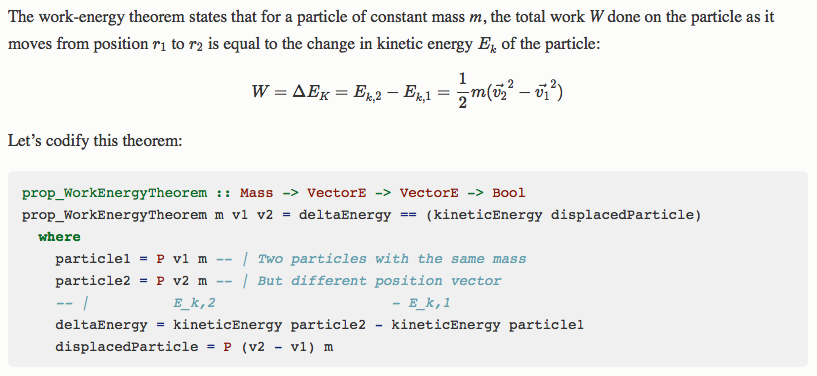
\includegraphics[width=1\textwidth]{figure/komposit-Ex.png}}
%   \caption{Implementation av relationen arbete-energi i läromaterialet}
%   \label{fig:komposit-ex}
% \end{figure}

% \section{Skapande av och publicering på hemsidan}
%
% Läromaterialet kompilerades med hjälp av ett skript och
% publicerades på en hemsida. Skriptet anropar
% Pandoc för att konvertera från källkod i Literate
% Haskell-format till HTML, redo att visas på en hemsida. Pandoc
% paketerar även med \textit{MathJax} som använder JavaScript för att
% rendera matematiska formler i LaTeX-format på fint och läsbart
% vis. Utan stöd för JavaScript skrivs matematik ut som omodifierad
% LaTeX-kod, vilket är mer svårläst, men fortfarande tolkningsbart. Det
% skrevs även CSS-kod för att modifiera utseendet av
% hemsidan för att den skulle bli prydligare och mer lättläst.
%
% Varje källfil betraktades som ett kapitel och publicerades som en
% separat undersida. Med hjälp av ett index beskrivet i skriptet
% konstruerades navigationselement mellan kapitel på varje undersida
% och en innehållsförteckning.
%
% För publicering lades all data producerad av skriptet i en ny git-gren (engelska \textit{git branch}) med namnet \texttt{gh-pages}. Att alla grenar synkroniseras
% mot GitHub medför att alla filer på \texttt{gh-pages} grenen
% visas som en hemsida med hjälp av \textit{GitHub
%   Pages}. Publiceringen skedde inte kontinuerligt eller automatiskt,
% utan krävde en manuell synkronisering vid varje önskad uppdatering av
% hemsidan.

\section{Möten och återkoppling}

  % Återkoppling från examinator (NAD): "Nils Anders Danielsson <nad@cse.gu.se>
  % 27 Feb (1 day ago)
  % to Patrik, Andreas
  % Hi,Your BSc project groups both try to make tools for learning. I had some
  % discussion with Andreas' group about their plans for evaluating how well
  % their product works. My position is that, given the resource limits of
  % these projects (and general problems of reproducibility in social
  % sciences), it is very hard to perform an evaluation that gives useful
  % results. I don't mind if your groups try to perform some kind of
  % evaluation, but I suggest that you tell them to avoid overstating the
  % importance of the evaluations in the final reports."
  % Jag tror det är kompatibelt med det jag sagt tidigare - att göra en "ordentlig" utvärdering av det pedagogiska utfallet är komplicerat och tar (kalender-)tid.
  % Informell utvärdering av en testgrupp bör dock ingå.

För att få återkoppling på läromaterialet hölls ett kort och informellt möte med
en testgrupp. Testgruppen bestod av tre andra studenter på Chalmers som gick
tredje året på Datateknik och Informationsteknik. De hade alla klarat kursen Fysik för
ingenjörer eller motsvarande och även klarat minst en kurs i Haskell.
Däremot hade de inte läst DSLsofMath eller motsvarande. Domänspecifika språk var
med andra ord nytt för dem. Under mötet gavs läromaterialet en kort presentation och bakgrund. Sedan fick de på egen hand läsa materialet och deras
spontana reaktioner och svar på frågor noterades.

Det hölls även två möten med Åke Fäldt. Ett möte hölls relativt
tidigt i projektet, 2018-03-02, och ett andra relativt sent, 2018-04-11.
Under mötena presenterades läromaterialet i sig och tanken med det, nämligen att
presentera fysik ur ett annat perspektiv, ett
programmeringsperspektiv. Diskussionen kretsade sedan kring svåra områden i Fysik för
ingenjörer, vad läromaterialet skulle kunna
bidra med för kunskaper till studenter samt dess eventuella roll i relation till
fysikkursen.
